\chapter{Cinematica Differenziale}
Fino adesso, abbiamo esaminato il problema della \emph{cinematica diretta} posizionale e successivamente \emph{l'inversione} della cinematica diretta. La \emph{cinematica differenziale} riguarda la derivazione della relazione che esiste tra le velocità dei giunti ed il moto dell'organo terminale (inteso come velocità di traslazione di un suo punto e velocità angolare).

\begin{align}
	KIN: \quad \underline{q} \longrightarrow \underline{p}, R \;(oppure\; \underline{p}, \underline{\phi}) \\
	\dot{KIN}: \quad \dot{\underline{q}} \longrightarrow \dot{\underline{p}}, \underline{\omega}\;(oppure\; \dot{\underline{p}}, \dot{\underline{\phi}})
\end{align}
	
\subsubsection{Cinematica diretta}
Nella trattazione della cinematica diretta si fissa una terna sull'organo terminale e si ricava la relazione tra le coordinate di giunto e la matrice di trasformazione omogenea $T_n^0$. In alternativa si può cercare la relazione esistente tra le coordinate di giunto ed il vettore $\underline{x}$ che definisce la posizione dell'organo terminale nello spazio operativo.

\subsubsection{Cinematica Differenziale}
Nello studio della cinematica differenziale bisogna invece cercare il legame tra le derivate temporali delle coordinate di giunto e la velocità della terna utensile, fissata all'organo terminale.

\section{Jacobiano Analitico}
Per tracciare la \emph{posizione} dell'organo terminale usiamo il \emph{vettore dello spazio operativo} $\underline{x}$ e derivando otteniamo il \emph{vettore velocità nello spazio operativo} $\dot{\underline{x}}$:

\begin{equation}
	\underline{x} = 
	\begin{bmatrix}
		\underline{p} \\
		\underline{\phi} \\
	\end{bmatrix}
	\qquad \dot{\underline{x}} = 
	\begin{bmatrix}
		\dot{\underline{p}} \\
		\dot{\underline{\phi}} \\
	\end{bmatrix}
\end{equation}

indicando con $\underline{p}$ posizione dell'origine della terna utensile e $\underline{\phi}$ una rappresentazione minima dell'orientazione.

Sia $\underline{f}$ la funzione $KIN$, consideriamo $\underline{x} = f(\underline{q})$ e definiamo la derivata del \emph{vettore dello spazio operativo} come segue:
\begin{equation}
	\dot{\underline{x}} =   \frac{\partial \underline{f}(\underline{q})}{\partial \underline{q}} \cdot \underline{\dot{q}}
\end{equation}

\paragraph{}
A questo punto, definiamo lo \emph{Jacobiano Analitico}, ovvero la \emph{matrice Jacobiana} $J_{a}$, come:
\begin{equation}
	J_a(\underline{q}) = \frac{\partial \underline{f}(\underline{q})}{\partial \underline{q}}
\end{equation}

pertanto possiamo scrivere:
\begin{equation}
	\dot{\underline{x}} = J_a(\underline{q}) \cdot \dot{\underline{q}} \quad \Rightarrow \quad 
	\begin{cases}
		\dot{\underline{p}} = J_{ap}(\underline{q})\,\underline{\dot{q}} \\
		\dot{\underline{\phi}} = J_{ao}(\underline{q})\,\dot{\underline{q}} \\
	\end{cases} 
\end{equation}

dove $J_{ap}$ e $J_{ao}$ sono le due sottomatrici ($\in\mathbb{R}^{3\times n}$) responsabili rispettivamente del cambiamento di posizione e del cambiamento di orientazione. Ottenendo:
\begin{equation}
	J_a(\underline{q}) = 
	\begin{bmatrix}
		J_{ap}(\underline{q}) \\
		J_{ao}(\underline{q})\\
	\end{bmatrix}
\end{equation}

notiamo che $J_a\in\mathbb{R}^{6 \times n}$ non è unico perchè dipende dalla particolare rappresentazione dell'orientazione. 
\paragraph{}
Lo \emph{Jacobiano Analitico} esprime un legame lineare tra $\dot{\underline{x}}$ e $\dot{\underline{q}}$, ovvero, esprime la relazione lineare tra la velocità nello \emph{spazio operativo} e quella nello \emph{spazio dei giunti}. Notiamo che anche se esprime una relazione lineare, lo $J_a$ è una funzione fortemente non lineare.

\subsection{Calcolo di $J_a$}
Il metodo standard di calcolare $J_a$ non è quello della definizione, vediamo di calcolarlo per un manipolatore planare 3R.

\begin{center}
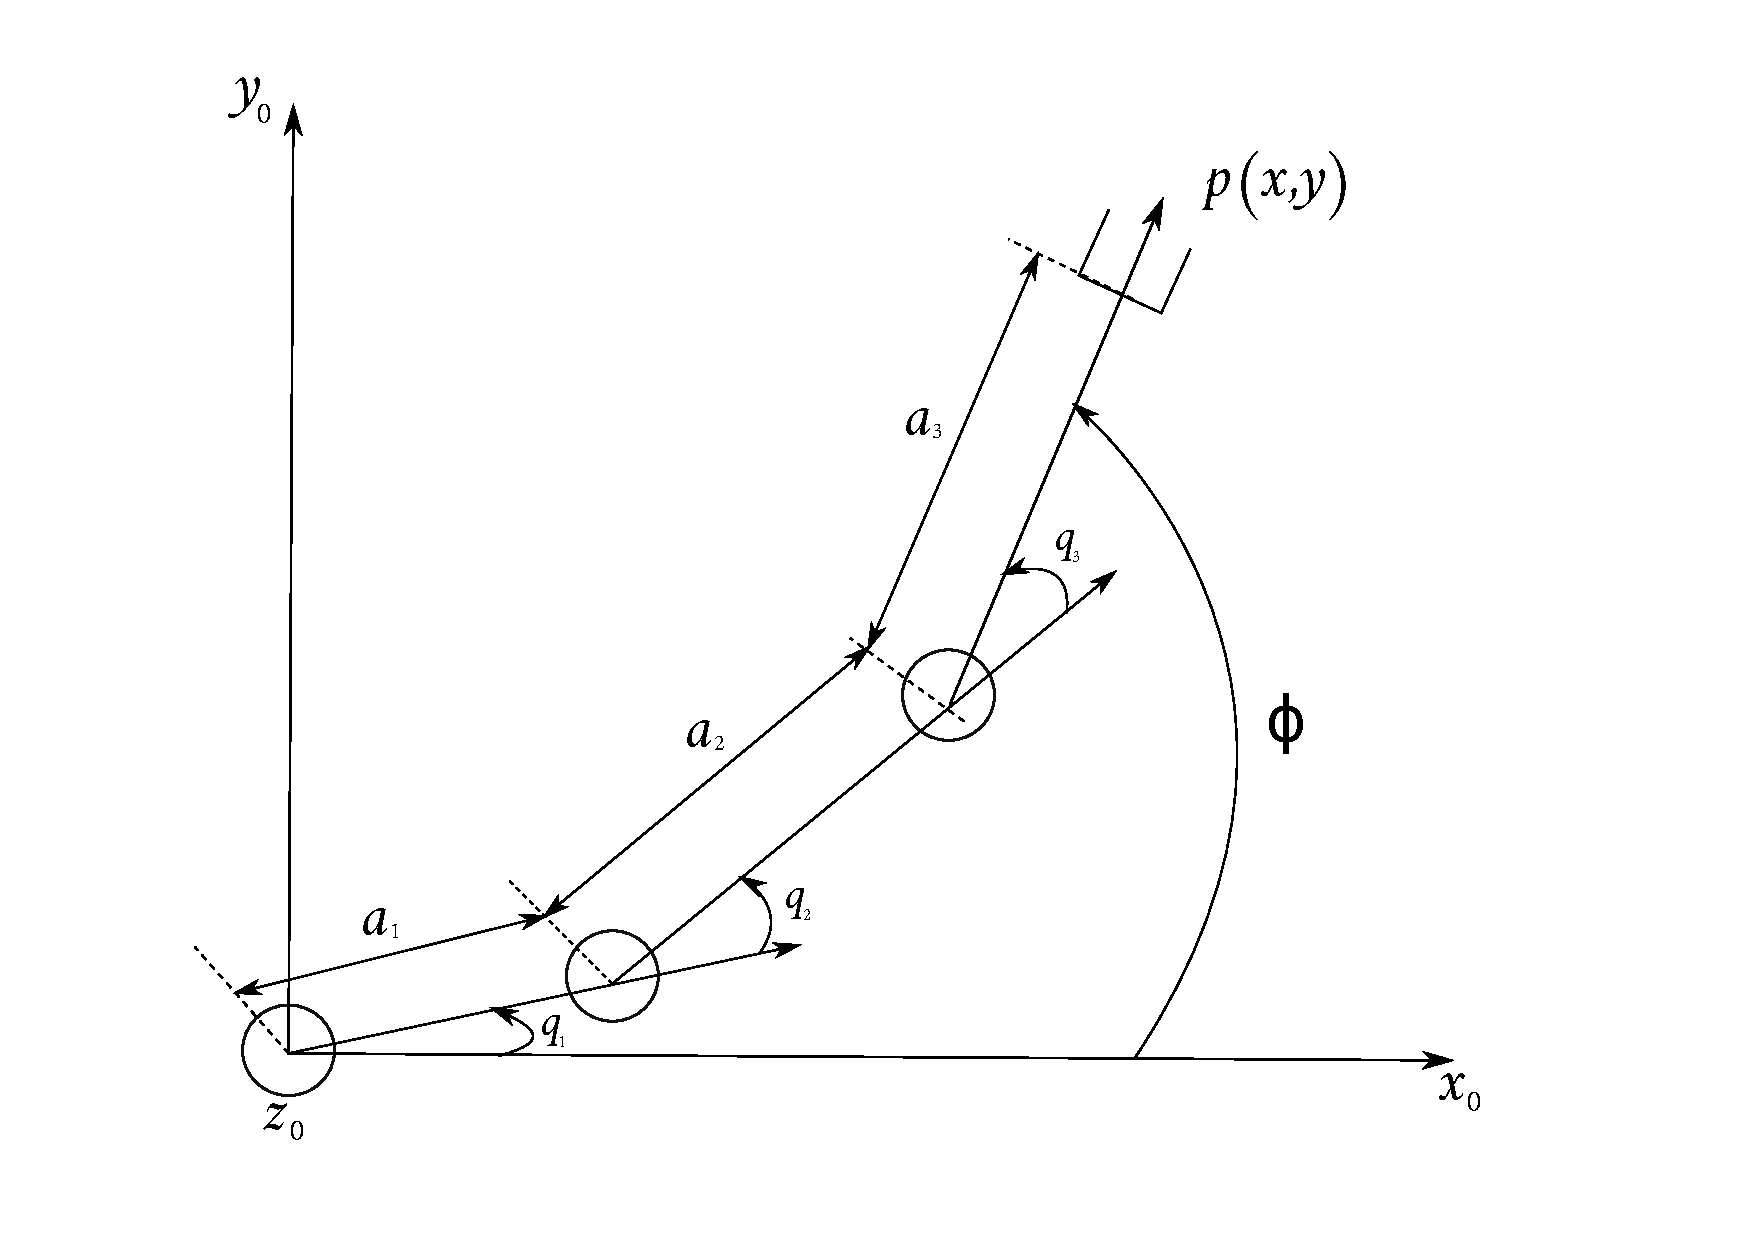
\includegraphics[scale=0.3]{manipolatore3RDiff.pdf}
\end{center}

\begin{equation}
	\underline{x} = \underline{f}(\underline{q}) \,=\,
	\begin{cases}
		x = a_1\,C_1 + a_2\,C_{12} + a_3\,C_{123} \\
		y = a_1\,S_1 + a_2\,S_{12} + a_3\,S_{123} \\
		\phi = q_1 + q_2 + q_3 \\
	\end{cases}
\end{equation}

a questo punto, deriviamo:
\begin{equation}
	\dot{\underline{x}} =   \frac{\partial \underline{f}(\underline{q})}{\partial \underline{q}} \cdot \underline{\dot{q}} = 
	\begin{cases}
		\dot{x} = \frac{\partial x}{\partial q_1} \dot{q_1} + \frac{\partial x}{\partial q_2} \dot{q_2} + \frac{\partial x}{\partial q_3} \dot{q_3} \\
		\dot{y} = \frac{\partial y}{\partial q_1} \dot{q_1} + \frac{\partial y}{\partial q_2} \dot{q_2} + \frac{\partial y}{\partial q_3} \dot{q_3} \\
		\dot{\phi} = \frac{\partial \phi}{\partial q_1} \dot{q_1} + \frac{\partial \phi}{\partial q_2} \dot{q_2} + \frac{\partial \phi}{\partial q_3} \dot{q_3} \\
	\end{cases}
\end{equation}

ovvero:
\begin{equation}
	\begin{bmatrix}
		\dot{x} \\
		\dot{y} \\
		\dot{\phi} \\
	\end{bmatrix}
	= 
	\begin{bmatrix}
		\frac{\partial x}{\partial q_1} & \frac{\partial x}{\partial q_2} & \frac{\partial x}{\partial q_3} \\
		\frac{\partial y}{\partial q_1} & \frac{\partial y}{\partial q_2} & \frac{\partial y}{\partial q_3} \\
		\frac{\partial \phi}{\partial q_1} & \frac{\partial \phi}{\partial q_2} & \frac{\partial \phi}{\partial q_3}
	\end{bmatrix}
	\cdot
	\begin{bmatrix}
		\dot{q_1} \\
		\dot{q_2} \\
		\dot{q_3} \\
	\end{bmatrix}
	\,\Rightarrow\,
	\begin{bmatrix}
		\dot{x} \\
		\dot{y} \\
		\dot{\phi} \\
	\end{bmatrix}
	= 
	J_a(q_1, q_2, q_3) \cdot
	\begin{bmatrix}
		\dot{q_1} \\
		\dot{q_2} \\
		\dot{q_3} \\
	\end{bmatrix}
\end{equation}

e pertanto, $J_a(\underline{q})$ risulta essere:
\begin{equation*}
	J_a(q_1, q_2, q_3) = 
	\begin{bmatrix}
		-(a_1\,S_1 + a_2\,S_{12} + a_3\,S_{123}) & -(a_2\,S_{12} + a_3\,S_{123}) & -a_3\,S_{123} \\
		a_1\,C_1 + a_2\,C_{12} + a_3\,C_{123} & a_2\,C_{12} + a_3\,C_{123} & a_3\,C_{123} \\
		1 & 1 & 1 \\
	\end{bmatrix}
\end{equation*}

\section{Jacobiano Geometrico}
La ($4.3$) ci fornisce una rappresentazione della \emph{velocità della terna utensile}, ma un'altra possibile descrizione è la seguente:
\begin{equation}
	\underline{v} = 
	\begin{bmatrix}
		\dot{\underline{p}} \\
		\underline{\omega} \\
	\end{bmatrix}
\end{equation}

dove $\dot{\underline{p}}$ indica la velocità di traslazione dell'origine della terna utensile rispetto alla terna base, mentre $\underline{\omega}$ è la velocità angolare della terna utensile, anch'essa relativamente alla terna base. Questa rappresentazione viene denominata \emph{screw di velocità}.

\paragraph{}
Con un ragionamento simile a quello di prima giungiamo alla seguente relazione matriciale:
\begin{equation}
	\underline{v} = J(\underline{q}) \cdot \dot{\underline{q}}
\end{equation}

definiamo $J(\underline{q}) \in \mathbb{R}^{6\times n}$ \emph{Jacobiano Geometrico} e mette in relazione lineare $\dot{\underline{q}}$ con $\underline{v}$. 

\paragraph{}
Otteniamo: 
\begin{equation}
	\underline{v} = 
	\begin{bmatrix}
		\underline{\dot{p}} \\
		\underline{\omega} \\
	\end{bmatrix}
	= J(\underline{q})\,\dot{\underline{q}} =
	\begin{bmatrix}
		J_p \\
		J_o \\
	\end{bmatrix}
	\cdot\underline{\dot{q}}
\end{equation}

quindi anche lo \emph{Jacobiano Geometrico} è composto da due sottomatrici $J_p \in\mathbb{R}^{3 \times n}$ e $J_o\in\mathbb{R}^{3 \times n}$ rispettivamente per la \emph{posizione} e per \emph{l'orientazione}.

pertanto:
\begin{equation}
	J = 
	\begin{bmatrix}
		J_p \\
		J_o \\
	\end{bmatrix}
	\, \Rightarrow \,
	\begin{cases}
		\underline{\dot{p}} = J_p \, \underline{\dot{q}} \\
		\underline{\omega} = J_o \, \underline{\dot{q}} \\
	\end{cases}
\end{equation}

\subsection{Calcolo di $J$}
Il calcolo dello Jacobiano geometrico $J$ si effettua considerando il contributo della velocità di ogni singolo giunto al moto dell'organo terminale, considerando tutti gli altri giunti bloccati, e sommando insieme tutti i contributi.

\paragraph{}
Ognuno dei contributi dei giunti al moto dell'organo terminale avrà un'espressione del tipo $\underline{J_i}\,\dot{q_i}$ dove $\underline{J_i}$ è la colonna \emph{i-esima} dello jacobiano. La velocità complessiva dell'organo terminale sarà quindi data da:

\begin{equation}
	\underline{v} = \sum_{i = 1}^{n} \underline{J_i}\,\dot{q_i} = 
	\begin{bmatrix}
		\,\underline{J_1} & \underline{J_2} & \cdots & \underline{J_n}\,
	\end{bmatrix}
	\begin{bmatrix}
		\dot{q_1} \\
		\dot{q_2} \\
		\vdots \\
		\dot{q_n}\\
	\end{bmatrix}
\end{equation}

per calcolare le colonne dello jacobiano, calcoliamo i vari contributi $\underline{J_i}\,\dot{q_i}$ distinguendo due casi: giunto $q_i$ \emph{rotoidale} e giunto $q_i$ \emph{prismatico}.

\subsubsection{Giunto Rotoidale}
Supponendo che il giunto \emph{i-esimo} sia rotoidale, una rotazione del giunto con velocità angolare $\dot{q_i}$, con tutti gli altri giunti bloccati, causerà una rotazione rigida della parte del robot che sta a valle del giunto $i$ attorno all'asse $z_{i-1}$ con velocità angolare espressa dal vettore: 
\begin{equation}
	\dot{q_i}\,\underline{k}_{i-1} 
\end{equation}
dove $\underline{k}_{i-1}$ è il versore del giunto $i$. Questo moto di rotazione attorno all'asse $z_{i-1}$ produce:
\begin{itemize}
	\item una velocità angolare dell'organo terminale, ovvero, del \emph{link n} pari a $\dot{q_i}\,\underline{k}_{\,i-1}$
	\item una velocità di traslazione del punto $\underline{p}$ pari a $\dot{q_i}\,\underline{k}_{\,i-1} \times (\,\underline{p} - \underline{O}_{\,i-1})$, dove $\underline{O}_{\,i-1}$ è il vettore posizione dell'origine della terna solidale al \emph{link i-1}
\end{itemize}

\begin{center}
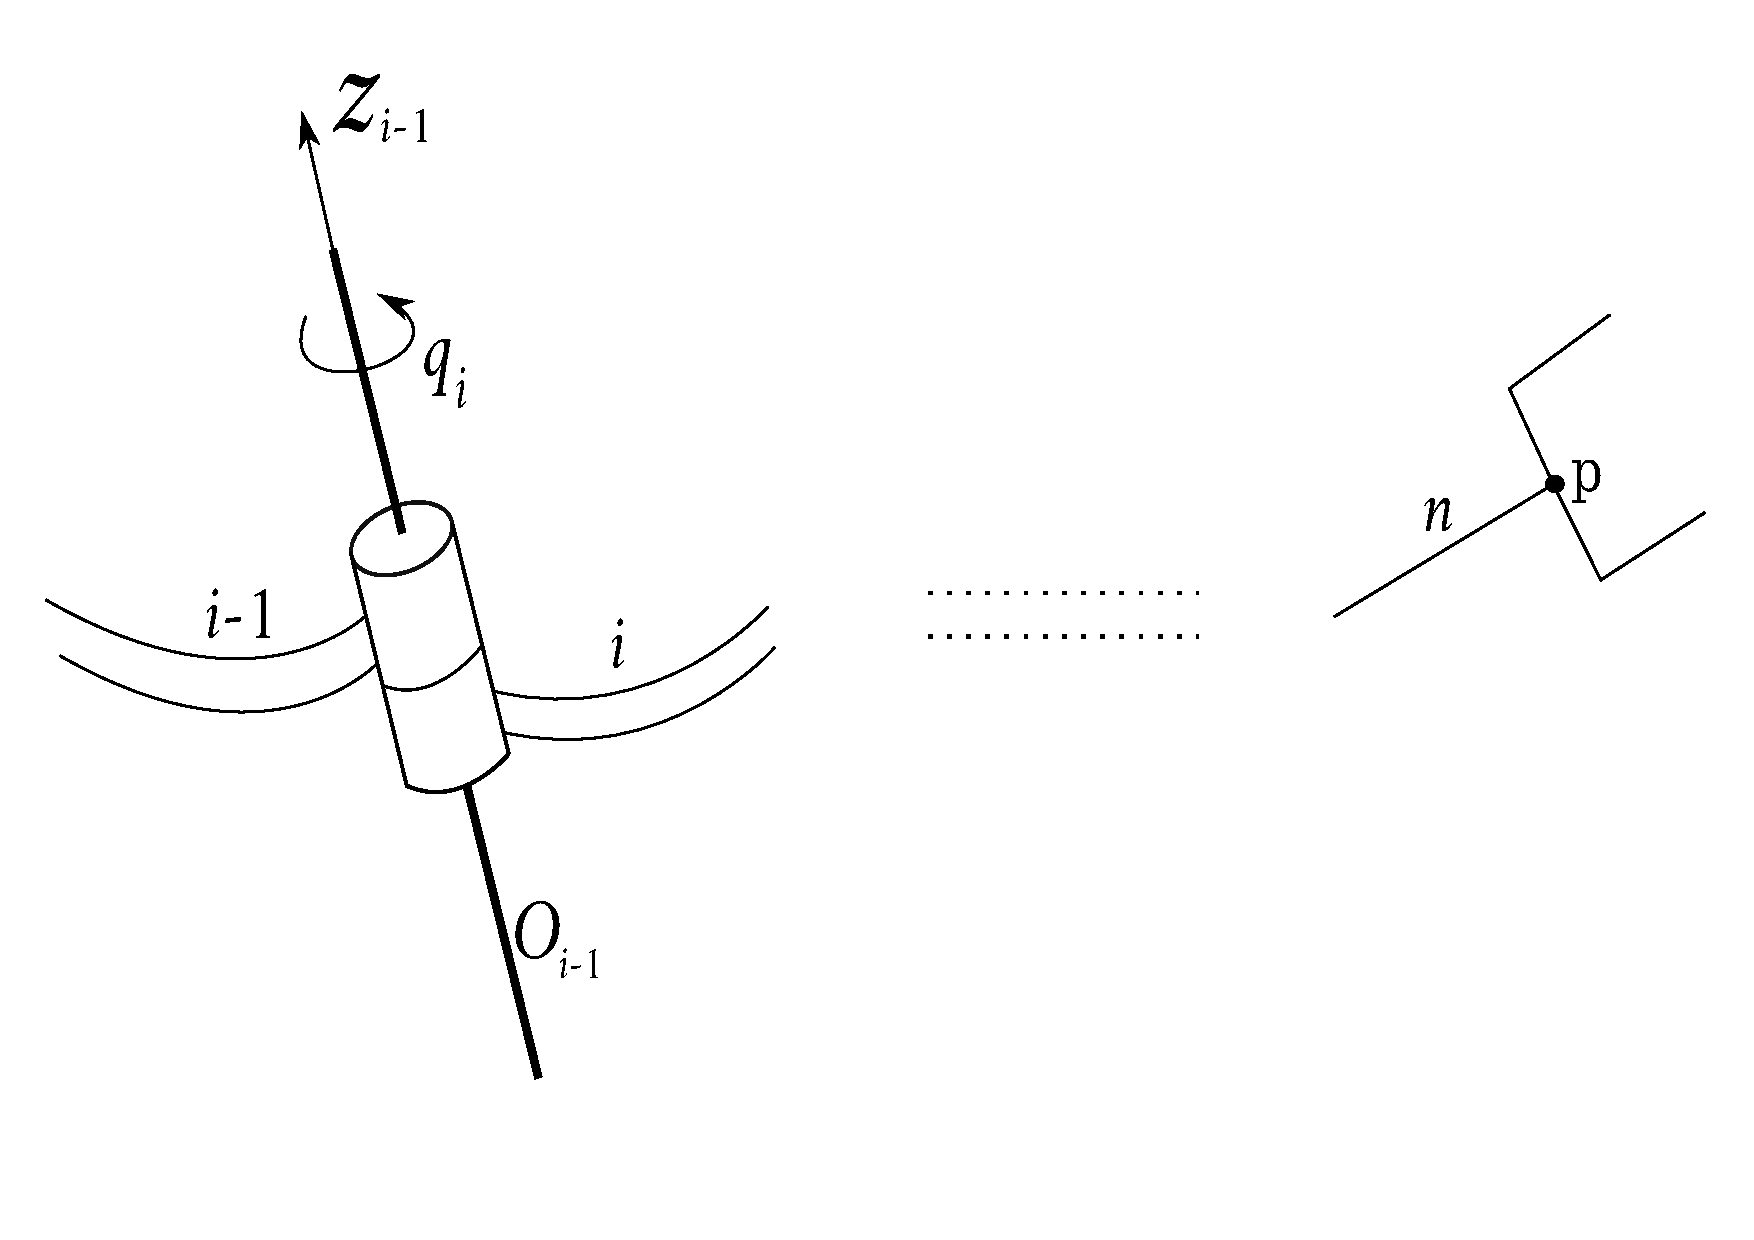
\includegraphics[scale=0.2]{giuntoRotoidale.pdf}
\captionof{figure}{Giunto rotoidale, i puntini indicano gli svariati giunti.}
\end{center}

\paragraph{}
Pertanto la colonna $\underline{J_i}$ dello jacobiano relativa al giunto $i$ risulta:
\begin{equation} \label{J_rotoidale}
	\underline{J}_{\,i} = 
	\begin{bmatrix}
		\underline{J}_{\,pi} \\
		\underline{J}_{\,oi} \\
	\end{bmatrix}
	= 
	\begin{bmatrix}
		\underline{k}_{\,i-1} \times (\,\underline{p} - \underline{O}_{\,i-1}) \\
		\underline{k}_{\,i-1}
	\end{bmatrix}
\end{equation}

\subsubsection{Giunto Prismatico}
Supponendo che il giunto \emph{i-esimo} sia prismatico, una traslazione del giunto con velocità $\dot{q_i}$, con tutti gli altri giunti bloccati, causerà una traslazione rigida della parte del robot che sta a valle del giunto $i$ lungo la direzione dell'asse $z_{i-1}$, con velocità angolare espressa dal vettore:
\begin{equation}
	\dot{d_i}\underline{k}_{\,i-1}
\end{equation}
dove $\underline{k}_{\,i-1}$ è il versore del giunto $i$. Tale moto di traslazione parallelo all'asse $z_{\,i-1}$ si traduce in:
\begin{itemize}
	\item un contributo nullo alla velocità angolare dell'organo terminale, ovvero del \emph{link n}
	\item un contributo alla velocità di traslazione del punto $\underline{p}$ pari a $\dot{d_i}\,\underline{k}_{\,i-1}$
\end{itemize}

\begin{center}
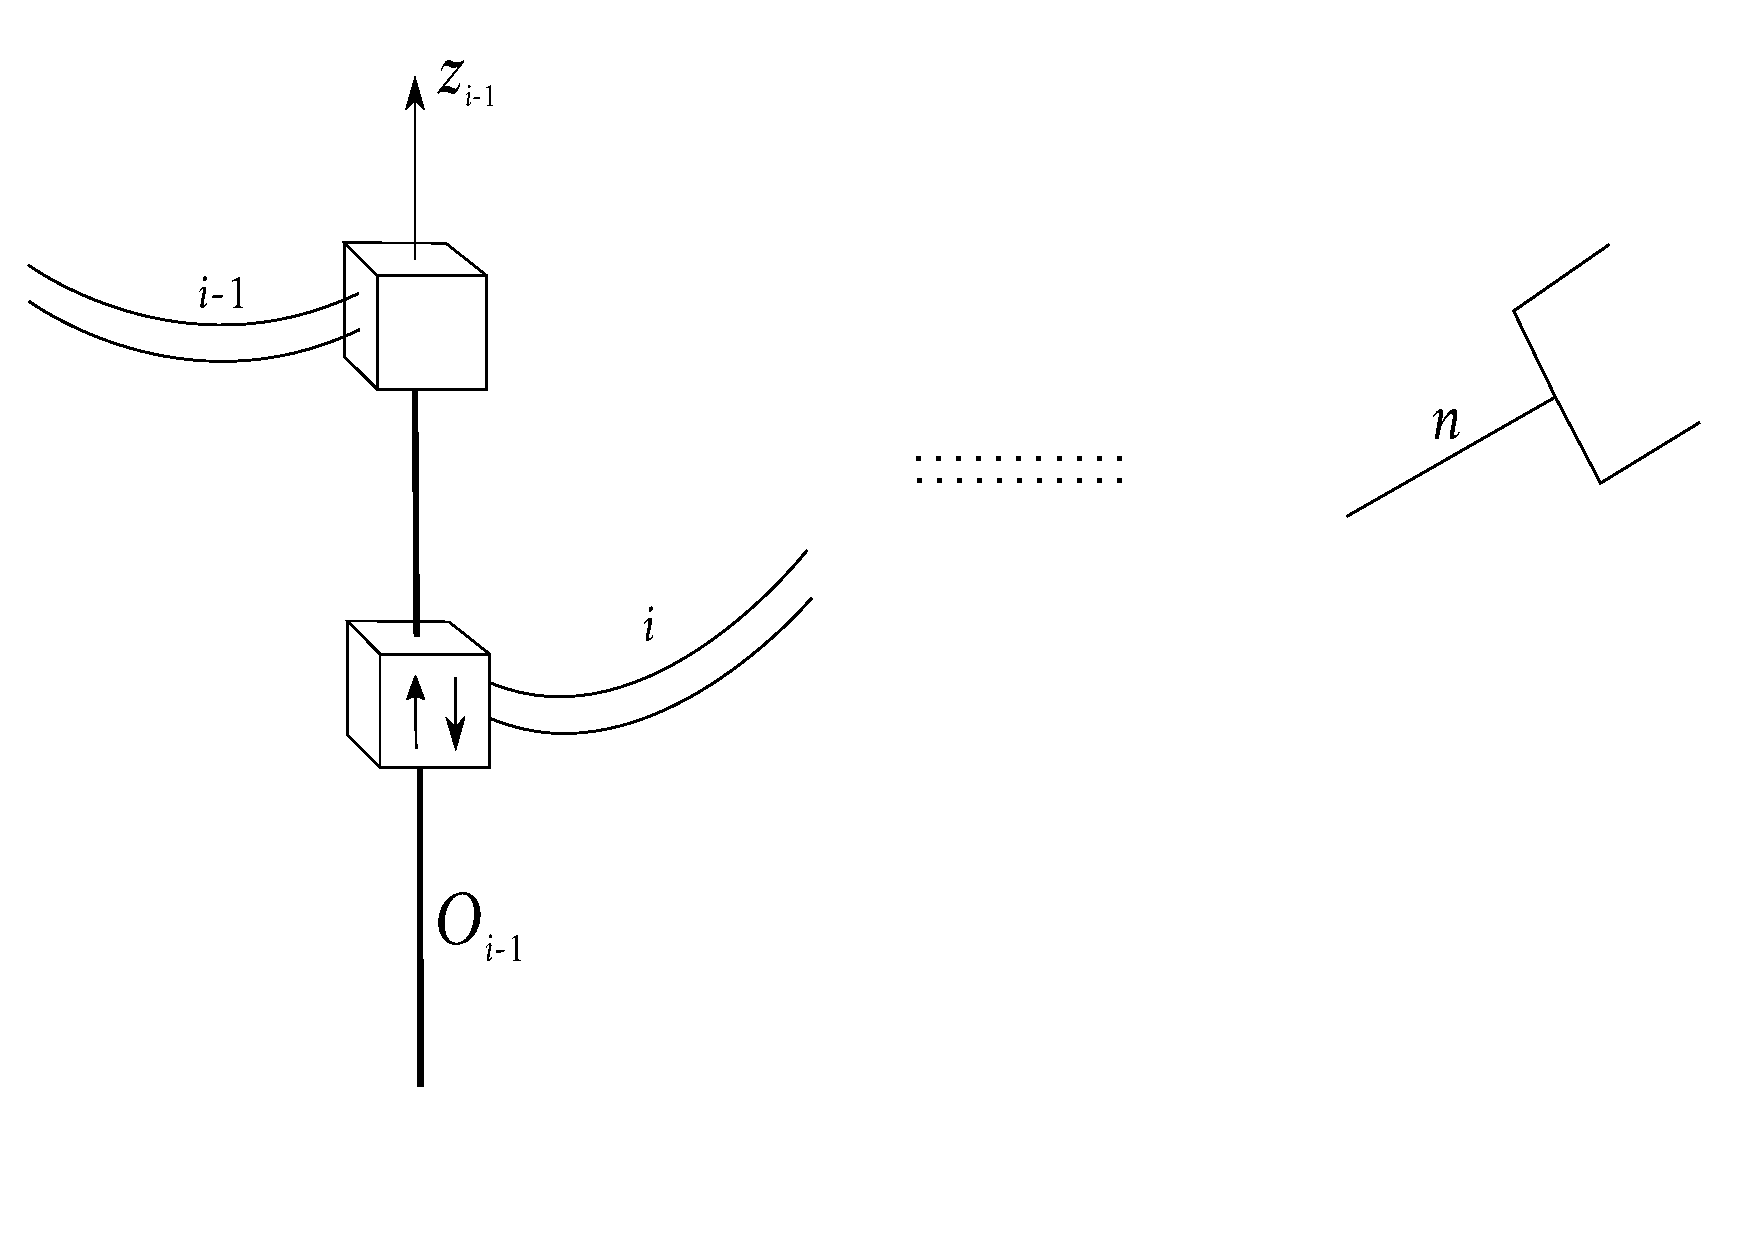
\includegraphics[scale=0.2]{giuntoPrismatico.pdf}
\captionof{figure}{Giunto prismatico, i puntini indicano gli svariati giunti.}
\end{center}

\paragraph{}
Pertanto la colonna $J_i$ dello jacobiano relativa al giunto $i$ risulta:
\begin{equation} \label{J_prismatico}
	\underline{J}_{\,i} = 
	\begin{bmatrix}
		\underline{J}_{\,pi} \\
		\underline{J}_{\,oi} \\
	\end{bmatrix}
	= 
	\begin{bmatrix}
		\underline{k}_{\,i-1} \\
		0 \\
	\end{bmatrix}
\end{equation}

\section{Relazione tra $J_a$ e $J$}
Esaminando la \eqref{J_rotoidale} e la \eqref{J_prismatico} notiamo che in generale vale $J_a \neq J$, ovvero, lo Jacobiano analitico è diverso dallo Jacobiano geometrico. Ma notiamo anche:
\begin{itemize}
	\item le parti traslazionali dei due Jacobiani coincidono: $J_{ap} = J_p$
	\item le parti rotazionali dei due Jacobiani differiscono: $J_{ao} \neq J_o$, perché $\underline{\omega} \neq \underline{\dot{\phi}}$
\end{itemize}

\paragraph{}
Cerchiamo il legame esistente tra $J_{ao}$ e $J_o$ nel caso in cui la rappresentazione dell'orientazione utilizzata sia quella di \emph{Eulero} $ZYZ$. Determiniamo il legame tra la velocità angolare di un corpo rigido e le derivate temporali degli angoli di Eulero che ne descrivono l'orientazione. Sfruttiamo il fatto che se ho $n+1$ corpi rigidi in moto ognuno rispetto al precedente allora:
\begin{equation} \label{omega}
	^0\underline{\omega}_{\,n,0} = \,^0\underline{\omega}_{\,1,0} + \,^0\underline{\omega}_{\,2,1} + \cdots + \,^0\underline{\omega}_{\,n,n-1}
\end{equation}

dove $^0\underline{\omega}_{\,i,i-1}$ è la \emph{velocità angolare} della terna $\langle i \rangle$ rispetto alla terna $\langle i-1 \rangle$ espressa in terna $\langle 0 \rangle$.

\paragraph{}
Esaminando le 4 terne di Eulero e le loro tre rotazioni:

\begin{center}
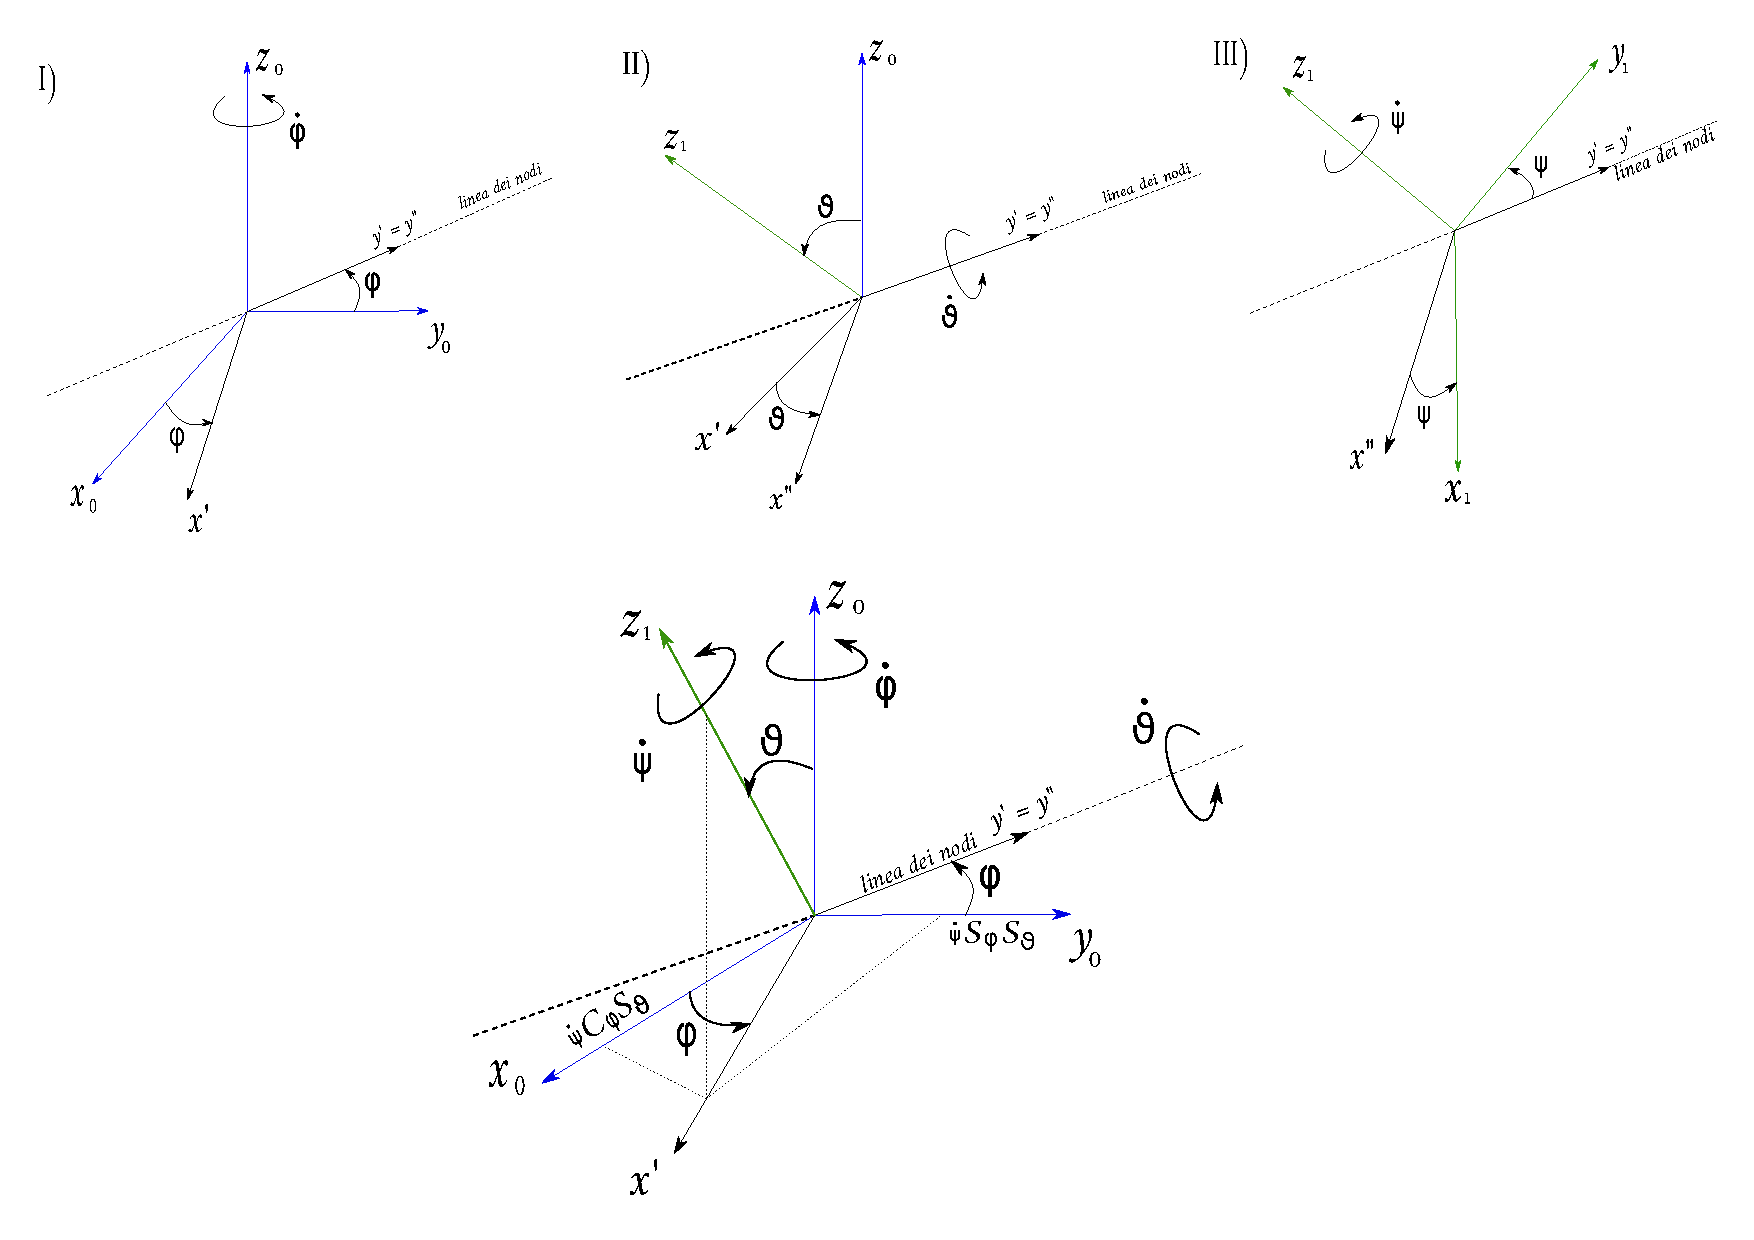
\includegraphics[scale=0.35]{rotazioniEuleroDiff.pdf}
\captionof{figure}{Le tre rotazioni di Eulero}
\end{center}

otteniamo:
\begin{equation*}
I)\;\;\dot{\varphi}\,\underline{k}_{\,0} = \dot{\varphi}
\begin{bmatrix}
	0 \\
	0 \\
	1 \\
\end{bmatrix}
\qquad
II)\;\;\dot{\theta}\,\underline{j}' = \dot{\theta}
\begin{bmatrix}
	- S_{\varphi} \\
	C_{\varphi} \\
	0 \\
\end{bmatrix}
\qquad
III)\;\;\dot{\psi}\underline{k}_{\,1} = 
\dot{\psi}
\begin{bmatrix}
	S_{\theta}C_{\varphi} \\
	S_{\theta}S_{\varphi} \\
	C_{\theta} \\
\end{bmatrix}
\end{equation*}

dove con $I)$, $II)$ e $III)$ indico le tre rotazioni.
\paragraph{}
Per quanto detto prima \eqref{omega}, possiamo esprimere la velocità angolare dell'ultima terna rispetto alla prima come la somma delle velocità angolari relativa di ogni terna rispetto alla precedente:
\begin{equation}
	\underline{\omega}=\dot{\varphi}\,\underline{k}_{\,0} + \dot{\theta}\,\underline{j}' + \dot{\psi}\underline{k}_{\,1} = 
	\begin{bmatrix}
		\underline{k}_{\,0} & \underline{j}' & \underline{k}_{\,1}
	\end{bmatrix}
	\begin{bmatrix}
		\dot{\varphi} \\
		\dot{\theta} \\
		\dot{\psi} \\
	\end{bmatrix}
\end{equation}

otteniamo:
\begin{equation}
	\underline{\omega} = T(\underline{\phi}) \cdot \dot{\underline{\phi}} \quad \text{con} \quad T(\underline{\phi}) = 
	\begin{bmatrix}
		\underline{k}_{\,0} & \underline{j}' & \underline{k}_{\,1} 
	\end{bmatrix}
	\quad \text{e} \quad \dot{\underline{\phi}} = 
	\begin{bmatrix}
		\dot{\varphi} \\
		\dot{\theta} \\
		\dot{\psi} \\
	\end{bmatrix}
\end{equation}

pertanto:
\begin{equation}
	T(\underline{\phi}) = 
	\begin{bmatrix}
		\underline{k}_{\,0} & \underline{j}' & \underline{k}_{\,1} 
	\end{bmatrix} = 
	\begin{bmatrix}
		0 & -S_{\varphi} & S_{\theta}C_{\varphi} \\
		0 & C_{\varphi} & S_{\theta}C_{\varphi} \\
		1 & 0 & C_{\theta} \\
	\end{bmatrix}
\end{equation}
\paragraph{}
Notiamo:
\begin{itemize}
	\item se siamo in \emph{singolarità di rappresentazione}, ovvero, $S_{\theta} = 0$ allora\\ 
	$det(T(\underline{\phi})) = 0$ e quindi $T(\underline{\phi})$ non è invertibile.
	\item se invece $det(T(\underline{\phi})) \neq 0$ allora la ($4.22$) può essere invertita: \begin{equation}
		\underline{\dot{\phi}} = T(\underline{\phi})^{-1} \cdot \underline{\omega}
	\end{equation}
\end{itemize}
\subsection{Calcolo di $J$ partendo da $J_a$ e viceversa}
Adesso consideriamo l'espressione di $\underline{\dot{\phi}}$ della ($4.6$) e andiamola a sostituire nella ($4.22$), otteniamo, considerando l'espressione di $\underline{\omega}$ della ($4.14$), due forme della $\underline{\omega}$ che possiamo eguagliare ottenendo:
\begin{equation}
	\begin{cases}
		\underline{\dot{\phi}} = J_{ao}\,\underline{\dot{q}} \\
		\underline{\omega} = T(\underline{\phi})\underline{\dot{\phi}}
	\end{cases}
	\;\Rightarrow\; 
	\begin{cases}
		\underline{\omega} = T(\underline{\phi})\,J_{ao}\,\underline{\dot{q}}\\
		\underline{\omega} = J_o \, \underline{\dot{q}} 
	\end{cases}
	\;\Rightarrow\;\;
	J_o = T(\underline{\phi})\,J_{ao}
\end{equation}
Se non siamo in singolarità di rappresentazione e quindi $S_{\theta} \neq 0$, possiamo invertire la relazione ottenendo:
\begin{equation}
	J_{ao} = T(\underline{\phi})^{-1}\,J_o
\end{equation}
A questo punto considerando $J_p = J_{ap} = I_{3 \times 3}\,J_{ap} + 0_{3 \times 3}\,J_{ao}$, dove $0_{3 \times 3}$ è una matrice di zeri $3 \times 3$ possiamo scrivere:
\begin{equation}
	J = 
	\begin{bmatrix}
	J_p \\
	J_o \\
	\end{bmatrix}
	=
	\underbrace{ 
	\begin{bmatrix}
		I_{3 \times 3} & 0_{3 \times 3} \\
		0_{3 \times 3} & T(\underline{\phi}) \\
	\end{bmatrix}
	}_{T_a(\underline{\phi})}
	\begin{bmatrix}
		J_{ap} \\
		J_{ao} \\
	\end{bmatrix}
	= 
	T_a(\underline{\phi})\,J_a
\end{equation}

dove abbiamo definito la matrice $T_a(\underline{\phi})\in\mathbb{R}^{6 \times 6}$. 
\paragraph{}
Dato che $T(\underline{\phi})$ è invertibile ($S_{\theta} \neq 0$) allora anche $T_a(\underline{\phi})$ è invertibile, otteniamo quindi:
\begin{itemize}
	\item Calcolo di $J$ partendo da $J_a$, $\Rightarrow$ $J = T_a(\underline{\phi})\,J_a$
	\item Calcolo di $J_a$ partendo da $J$, $\Rightarrow$ $J_a = T_a(\underline{\phi})^{-1}\,J$ 
\end{itemize}

\section{Singolarità Cinematica}
Una \emph{Singolarità Cinematica}, da qui in avanti indicata con il termine \emph{singolarità} o \emph{"punto singolare"} è una configurazione in cui lo Jacobiano Geometrico $J$ (oppure $J_a$) perde rango. Per un manipolatore nello spazio a 6 DOF, il termine \emph{"full rank"} indica che lo Jacobiano ha rango 6. Chiaramente la \emph{"Singolarità Cinematica"} è diversa dalla \emph{"Singolarità di Rappresentazione"}. 
\paragraph{}
Classifichiamo le singolarità cinematiche:
\begin{itemize}
	\item \textbf{Singolarità di confine:} Si presentano nelle configurazioni in cui il manipolatore è completamente esteso o completamente ripiegato su se stesso. Non rappresentano un grosso inconveniente perché risultano visibili. Si chiamano \emph{di confine} perché sono ai confini del \emph{workspace}.
	\item \textbf{Singolarità interna:} Causate solitamente dall’allineamento di qualche asse di giunto. Sono un problema perchè possono interessare traiettorie di lavoro del manipolatore. Si chiamano così \emph{interne} perché sono dentro il \emph{workspace}.
\end{itemize}
\paragraph{}
In corrispondenza delle \emph{singolarità} si verificano le seguenti circostanze di notevole interesse, perchè potenzialmente pericolose:
\begin{itemize}
	\item il manipolatore perde mobilità in certe direzioni
	\item possono esistere infinite soluzioni al problema cinematico
	\item in vicinanza delle singolarità, per far eseguire all'organo terminale piccoli \emph{screw di velocità} $\underline{v}$, i giunti del manipolatore devono muoversi con velocità molto elevate
\end{itemize} 

\subsection{Studio di singolarità}
Lo \emph{studio di singolarità} consiste nel cercare tutte le possibili configurazioni singolari di un dato manipolatore. Tale studio in generale non è facile e l'identificazione di tutte le singolarità di una data struttura di manipolazione non sempre è nota in forma chiusa. 
\paragraph{}
Un valore che ci è utile valutare per tale studio è \emph{l'indice di manipolabilità} $\sqrt{m}$ con $m = det(JJ^T)$, infatti, se $J$ perde rango, la matrice quadrata (e simmetrica) $JJ^T$ diventa singolare, ovvero con il determinante nullo.
\paragraph{}
Consideriamo $n$ il numero di gradi di libertà e supponiamo che il numero di variabili dello spazio operativo che servono per eseguire un determinato compito sia $r$, otteniamo:
\begin{equation}
	\underline{v} = J\,\underline{\dot{q}}, \quad \underline{\dot{q}}\in\mathbb{R}^n, \; \underline{v}\in\mathbb{R}^r
\end{equation}
Se $r<n$, il manipolatore risulta \emph{ridondante} da un punto di vista cinematico ed esistono $(n-r)$ gradi di libertà ridondanti. 

\paragraph{}
Lo Jacobiano caratterizza la trasformazione lineare dallo spazio delle velocità dei giunti allo spazio delle velocità dell'organo terminale. La trasformazione è illustrata in figura ($4.4$).
\begin{center}
\includegraphics[scale=0.35]{MappaturaCinDiff.pdf}
\captionof{figure}{Mappatura cinematica differenziale}
\end{center}
\paragraph{}
L'equazione cinematica differenziale ($4.28$) può essere caratterizzata in termini dell'\emph{immagine} e del \emph{nullo} della trasformazione, si ha che:
\begin{itemize}
	\item \emph{L'immagine} di J è il sottospazio $\mathcal{R}$(J) in $\mathbb{R}^r$ che individua le velocità dell'organo terminale che possono venir generate dalle velocità di giunto, nella configurazione assegnata al manipolatore.
	\item \emph{Il nullo} di J è il sottospazio $\mathcal{N}$(J) in $\mathbb{R}^n$ a cui appartengono le velocità di giunto che non producono alcuna velocità all'organo terminale, nella configurazione assegnata al manipolatore.
\end{itemize} 

\paragraph{}
Vale la seguente relazione:
\begin{equation}
	\text{dim}(\mathcal{R}(J)) + \text{dim}(\mathcal{N}(J)) = n
\end{equation}

Se lo Jacobiano è a \emph{rango pieno}, si ha: 
\begin{equation}
	\text{dim}(\mathcal{R}(J)) = r \qquad \text{dim}(\mathcal{N}(J)) = n-r
\end{equation}

Al contrario, se lo Jacobiano degenera in presenza di singolarità, la dimensione dell'\emph{immagine} diminuisce e allo stesso tempo aumenta quella del \emph{nullo}. Nei manipolatori ridondanti, si ha $\text{dim}(\mathcal{N}(J))>0$, essi prendono il nome di \emph{automoti}.

\subsubsection{Proiettori nel nullo di J}
Sia $P\in\mathbb{R}^{n \times n}$ si dice che è un \emph{proiettore} nel nullo di $J$ se: 
\begin{equation}
	\forall\underline{\dot{q}}\in\mathbb{R}^n \;\Rightarrow\; P\underline{\dot{q}}\in\mathcal{N}(J)
\end{equation}
supponiamo di avere una \emph{velocità desiderata} $\underline{v}_{\,des}$ e una $\underline{\dot{q}}$ tale da soddisfare 
\begin{equation}
	\underline{v}_{\,des} = J(\underline{q})\,\underline{\dot{q}}
\end{equation}
allora anche 
\begin{equation}
	\underline{\dot{q}} + P\,\underline{\dot{q}}_{\,a}
\end{equation}
con $\underline{\dot{q}}_{\,a}$ vettore arbitrario di \emph{velocità nello spazio dei giunti} è soluzione della ($4.32$), ovvero: 
\begin{equation}
	\underline{v}_{\,des} = J(\underline{\dot{q}} + P\,\underline{\dot{q}}_{\,a}) \qquad \forall \underline{\dot{q}}_{\,a}\in\mathbb{R}^n
\end{equation}

tale risultato è di importanza notevole per la risoluzione della ridondanza, poichè una soluzione del tipo ($4.33$) mette in luce la possibilità di scegliere il vettore $\underline{\dot{q}}_{\,a}$ in maniera tale da utilizzare vantaggiosamente i gradi di libertà ridondanti. In effetti, questo vettore arbitrario genera dei \emph{moti interni} della struttura che non apportano modifiche alla posa dell'organo terminale.

\subsection{Calcolo delle singolarità di struttura del manipolatore antropomorfo}
\paragraph{}
Esiste una classe di manipolatori a 6 DOF che semplifica il problema dello studio delle singolarità, si tratta di tutti i manipolatori dotati di \emph{polso sferico}. Per affrontare lo studio delle singolarità di un manipolatore con polso sferico e struttura portante (che può essere, ad esempio, antropomorfo, sferico o cilindrico), analizziamo lo Jacobiano geometrico $J$:

\begin{equation}
	J = 
	\begin{bmatrix}
		J_{1p} & J_{2p} & J_{3p} & J_{4p} & J_{5p} & J_{6p} \\
		J_{1o} & J_{3o} & J_{3o} & J_{4o} & J_{5o} & J_{6o} 
	\end{bmatrix}
	=
	\begin{bmatrix}
		J_{11} & J_{12} \\
		J_{21} & J_{22} \\
	\end{bmatrix}
	\quad \text{con} \quad J_{ij}\in\mathbb{R}^{3 \times 3}
\end{equation}
Se vogliamo $det(J_{12}) = \vert J_{12} \vert = 0$ oppure $\vert J_{21} \vert = 0$ allora:$\vert J \vert = \vert J_{11} \vert \cdot \vert J_{22} \vert$.
\paragraph{}
Per rendere nullo $\vert J_{12} \vert$, scegliamo di piazzare l’origine della terna utensile $\underline{O_6}$ nel \emph{centro del polso} $\underline{w}$, quindi otteniamo: $\vert J_{12} \vert = 0_{3 \times 3}$. Questo significa che possiamo studiare:
\begin{itemize}
	\item Gli zeri di $\vert J_{11} \vert$ (\emph{singolarità di struttura portante})
	\item Gli zeri di $\vert J_{22} \vert$ (\emph{singolarità di polso sferico})
\end{itemize}
procediamo con un esempio.
Calcoliamo le singolarità di struttura del manipolatore antropomorfo, per farlo, serviamoci della seguente figura:
\begin{center}
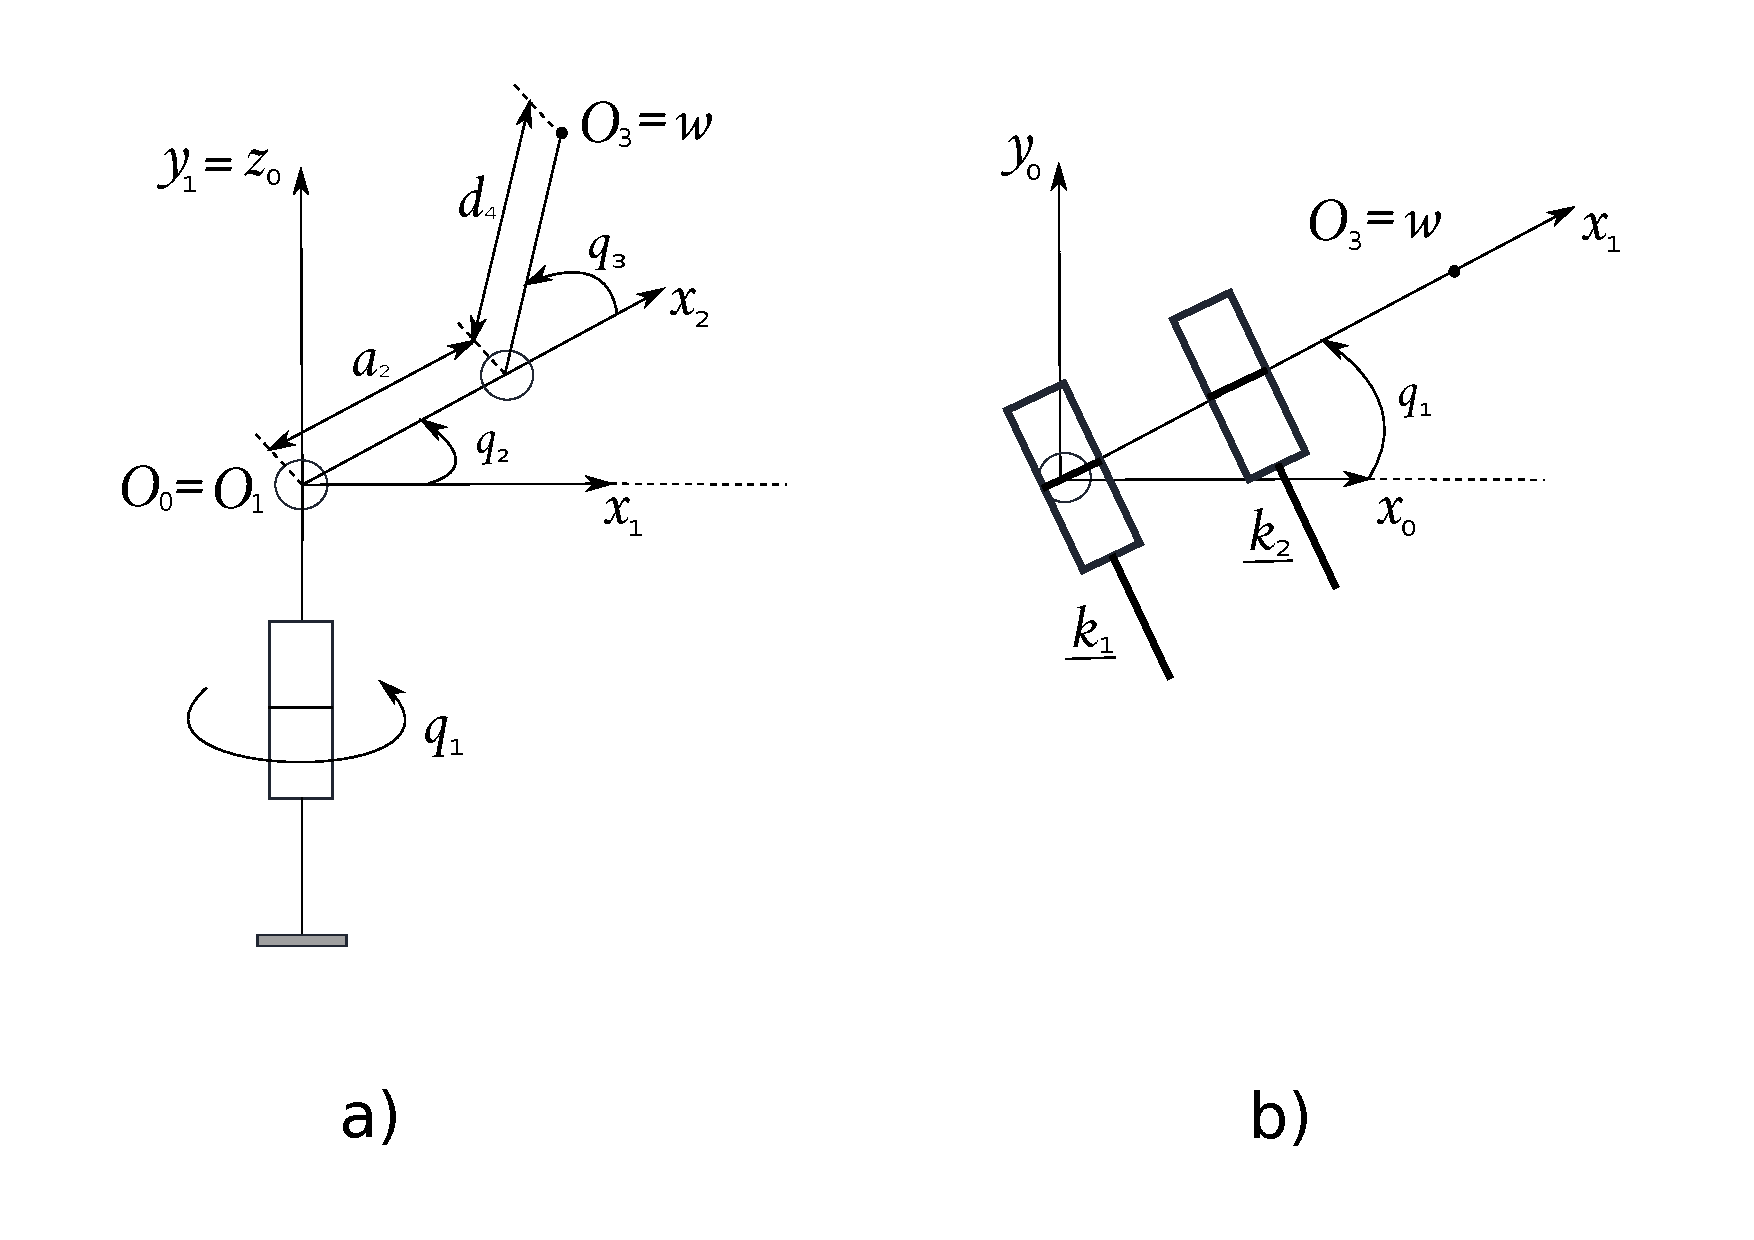
\includegraphics[scale=0.333]{visteManipolatoreDiff.pdf}
\captionof{figure}{vista in pianta: a) sul piano $x_1y_1$  b) sul piano $x_0y_0$}
\end{center}
Procediamo utilizzando due vie: quella geometrica e quella algebrica:

\subsubsection{Via Geometrica}
Si cerca di disegnare il manipolatore in configurazioni in cui una (o più) componenti di velocità di $w$ non sono realizzabili. Otteniamo:
\begin{itemize}
	\item si ha \emph{singolarità di gomito} quando $q_3 = 0$ (di confine)
	\item si ha \emph{singolarità di spalla} quando $w\in z_0\,\equiv\,y_1$ (interna), ovvero, quando $w_{x_1} = 0 = a_2C_2 + d_4C_{23} = 0$
\end{itemize}

esaminando il \emph{grado di mobilità} che si perde nei due casi:
\begin{itemize}
	\item Gomito: \emph{non} si può realizzare una velocità lungo $x_2$
	\item Spalla: \emph{non} si può realizzare una velocità in direzione $\perp$ al piano del braccio $x_1y_1$, cioè in direzione di $z_1 \parallel z_2$.
\end{itemize}

\subsubsection{Via Algebrica}
In linea generale, si cercano gli zeri di $J_{11}$. Iniziamo scrivendo $\underline{k_0}$, $\underline{k_1}$, $\underline{k_2}$:
\begin{equation}
	\underline{k_0} =
	\begin{bmatrix}
		0 & 0 & 1
	\end{bmatrix}^{T}
	\qquad \underline{k_1} =
	\begin{bmatrix}
		S_1 & -C_1 & 0
	\end{bmatrix}^{T}
	\qquad \underline{k_2} = \underline{k_1}
\end{equation}
adesso scriviamo $\underline{O_0}$, $\underline{O_1}$, $\underline{O_2}$, $\underline{O_3}$:
\begin{equation}
	\underline{O_0} = \underline{O_1} = 
	\begin{bmatrix}
		0 \\
		0 \\
		0 \\
	\end{bmatrix}
	\qquad \underline{O_2} =
	\begin{bmatrix}
		a_2C_1C_2 \\
		a_2S_1C_2 \\
		a_2S_2 \\
	\end{bmatrix}
	\qquad \underline{O_3} = w = 
	\begin{bmatrix}
		C_1(a_2C_2 + d_4C_{23}) \\
		S_1(a_2C_2 + d_4C_{23}) \\
		a_2S_2 + d_4S_{23} \\
	\end{bmatrix}
\end{equation}
possiamo scrivere adesso lo Jacobiano:
\begin{equation*}
	J_{11} = 
	\begin{bmatrix}
		\underline{k_0} \times (\underline{O_3} - \underline{O_0}) & \underline{k_1} \times (\underline{O_3} - \underline{O_1}) & \underline{k_2} \times (\underline{O_3} - \underline{O_2})
	\end{bmatrix}\in\mathbb{R}^{3 \times 3}
\end{equation*}

considerando che $\underline{O_0}$ e $\underline{O_1}$ sono nulli:
\begin{equation}
	J_{11} = 
	\begin{bmatrix}
		\underbrace{\underline{k_0} \times \underline{O_3}}_{\text{colonna 1}} & \underbrace{\underline{k_1} \times \underline{O_3}}_{\text{colonna 2}} & \underbrace{\underline{k_2} \times (\underline{O_3} - \underline{O_2})}_{\text{colonna 3}}
	\end{bmatrix}\in\mathbb{R}^{3 \times 3}
\end{equation}
\paragraph{}
Adesso andiamo a scrivere esplicitamente lo Jacobiano esprimendo il prodotto vettoriale con il formalismo matriciale introdotto a pagina $8$.
\begin{equation*}
	J_{11} = 
	\begin{bmatrix}
		\underbrace{
		\begin{bmatrix}
			0 & -1 & 0 \\
			1 & 0 & 0 \\
			0 & 0 & 0 \\
		\end{bmatrix}
		}_{S(\underline{k_0})}
		\underline{O_3} & 
		\underbrace{
		\begin{bmatrix}
			0 & 0 & -C_1 \\
			0 & 0 & -S_1 \\
			C_1 & S_1 & 0 \\
		\end{bmatrix}
		}_{S(\underline{k_1})}
		\underline{O_3} &
		\underbrace{
		\begin{bmatrix}
		0 & 0 & -C_1 \\
		0 & 0 & -S_1 \\
		C_1 & S_1 & 0 \\
		\end{bmatrix}
		}_{S(\underline{k_2})}
		(\underline{O_3} - \underline{O_2})
	\end{bmatrix}
\end{equation*}

considerando:
\begin{equation}
	(\underline{O_3} - \underline{O_2}) = 
	\begin{bmatrix}
		d_4C_1C_{23} \\
		d_4S_1C_{23} \\
		d_4S_{23} \\
	\end{bmatrix}
\end{equation}

a questo punto, svolgendo i prodotti matriciali considerando ($4.30$) e ($4.32$), otteniamo:
\begin{equation}
	J_{11} = 
	\begin{bmatrix}
		-S_1(a_2C_2 + d_4C_{23}) & -C_1(a_2S_2 + d_4S_{23}) & -C_1d_4S_{23} \\
		C_1(a_2C_2 + d_4C_23) & -S_1(a_2S_2 + d_4S_{23}) & -S_1d_4S_{23} \\
		0 & a_2C_2 + d_4C_{23} & d_4C_{23} \\
	\end{bmatrix}
\end{equation}
\paragraph{}
Calcoliamo il determinante $det(J_{11}) = \vert J_{11} \vert$ dello Jacobiano:
\begin{align*}
	\vert J_{11} \vert = -S_1(a_2C_2 + d_4C_{23})[-d_4S_1C_{23}(a_2S_2 + d_4S_{23}) + d_4S_1S_{23}(a_2C_2 + d_4C_{23})]- \\ 
	- C_1(a_2C_2 + d_4C_{23})[-d_4C_1C_{23}(a_2S_2 + d_4S_{23}) + d_4C_1S_{23}(a_2C_2 + d_4C_{23})] = \\
	= d_4S_1^2(a_2C_2 + d_4C_{23})[C_{23}(a_2S_2 + d_4S_{23}) - S_{23}(a_2C_2 + d_4C_{23})]+\\
	+ d_4C_1^2(a_2C_2 + d_4C_{23})[C_{23}(a_2S_2 + d_4S_{23}) - S_{23}(a_2C_2 + d_4C_{23})] = \\
	= d_4(a_2C_2 + d_4C_{23})[C_{23}(a_2S_2 + d_4S_{23}) - S_{23}(a_2C_2 + d_4C_{23})] = \\
	= d_4(a_2C_2 + d_4C_{23})[C_{23}a_2S_2 + C_{23}d_4S_{23} - a_2C_2S_{23} - d_4C_{23}S_{23}] = \\
	= d_4(a_2C_2 + d_4C_{23})[-a_2(S_{23}C_{2} - C_{23}S_2)] = \\
	= d_4(a_2C_2 + d_4C_{23})[-a_2\sin((q_2 + q_3) - q_2)] = \\
	= \underbrace{d_4(a_2C_2 + d_4C_{23})}_{\text{spalla}} \underbrace{[-a_2\sin(q_3)]}_{\text{gomito}}
\end{align*}\\\\\\


quindi otteniamo che il $\vert J \vert$ si annulla se:
\begin{itemize}
	\item $a_2C_2 + d_4C_{23} = 0$: il centro del polso si trova sull'asse del giunto 1, ovvero, sull'asse $z_0$. Il manipolatore perde mobilità nella direzione $z_1$. (\emph{singolarità di spalla})
	\item $S_3 = 0$: il link $2$ e $3$ sono allineati, il gomito è completamente steso ($q_3 = 0$) oppure completamente piegato ($q_3 = \pm\pi$). Il manipolatore perde mobilità nella direzione $x_2$. (\emph{singolarità di gomito})
\end{itemize}